\chapter{Introduction Sensor Fusion}
\label{chap:Intro}

For enabling a autonomous flight, the Raspberry Pi has to know the orientation. Figure \ref{fig:angles} shows the axes and the naming of the rotation around the axes. These rotations are later used for the calculation for the roll, pitch and yaw angles.

\begin{figure}[H]
	\centering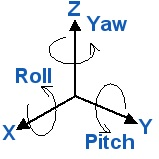
\includegraphics[width=0.3\textwidth]{fig/Roll_pitch_yaw}
	\caption{Roll, Pitch, Yaw \cite{doc:boreg}}
	\label{fig:angles}
\end{figure}

To get reliable stable orientation of the Raspberry Pi and so from the Quadrocopter several sensors can be used. Either a acceleration sensor, a magnetic sensor or a gyroscope can be used. But each of them have some drawbacks.\\
The acceleration sensor is very fast and delivers reliable pitch and roll angles, but the yaw angle itself can't be calculated. Another problem is, that due to vibrations a smooth angle is not possible to calculate.\\\\
The magnetometer can be used to calculate the heading, this means the yaw angle but not the roll and pitch angle. Another problem when the sensor has a roll and pitch angle, the heading can not be easily calculated. In this case a tilt compensation has to be done. In the figure \ref{fig:Mag_Acc} the logging of the pitch and roll angle calculated from the acceleration sensor and the yaw angle calculated with the magnetometer can be seen. When those sensors are not combined errors occur during the calculation. In the time from 250 seconds to 450 seconds a yaw angle is applied which leads just to a yaw angle change. In the time area from 500 seconds to 600 seconds a roll angle is applied which also leads to a yaw change which is an error. In the time area from 700 seconds to 800 seconds a pitch angle is applied which also leads to a yaw change which is an error.\\

\begin{figure}[H]
	\centering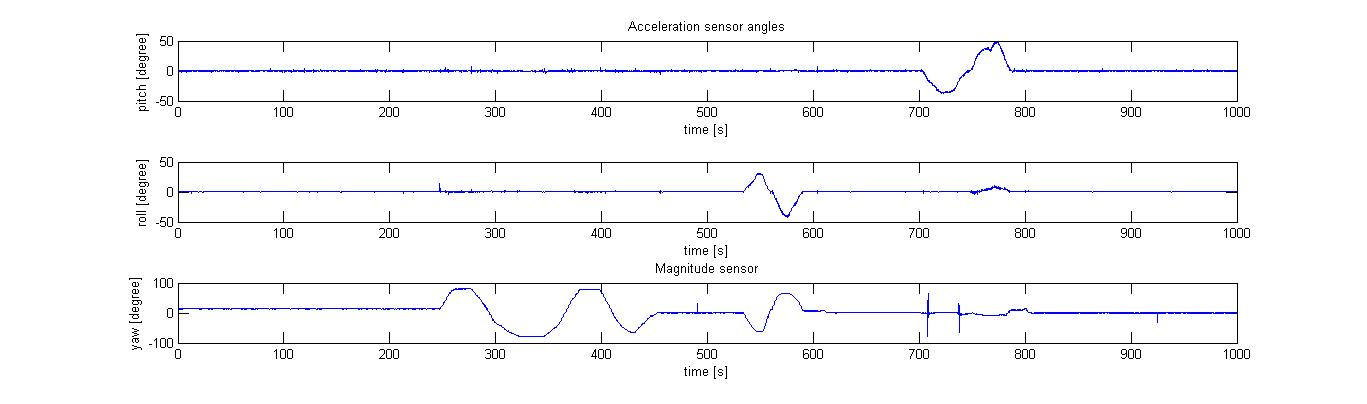
\includegraphics[width=1.0\textwidth]{fig/Magn_Acc.jpg}
	\caption{Magnitude / Acceleration angles}
	\label{fig:Mag_Acc}
\end{figure}

The last sensor is the gyroscope. The angle can be easily calculated by integrating the rates of the gyroscope. The sensor is not as fast as the acceleration sensor. So vibrations make no problems for the calculation. But due to the problem of the offset of the gyroscope, the angles will be drifting because of the integration of the rotation rates. This can be seen in figure \ref{fig:Comp_gyro}\\\\

\begin{figure}[H]
	\centering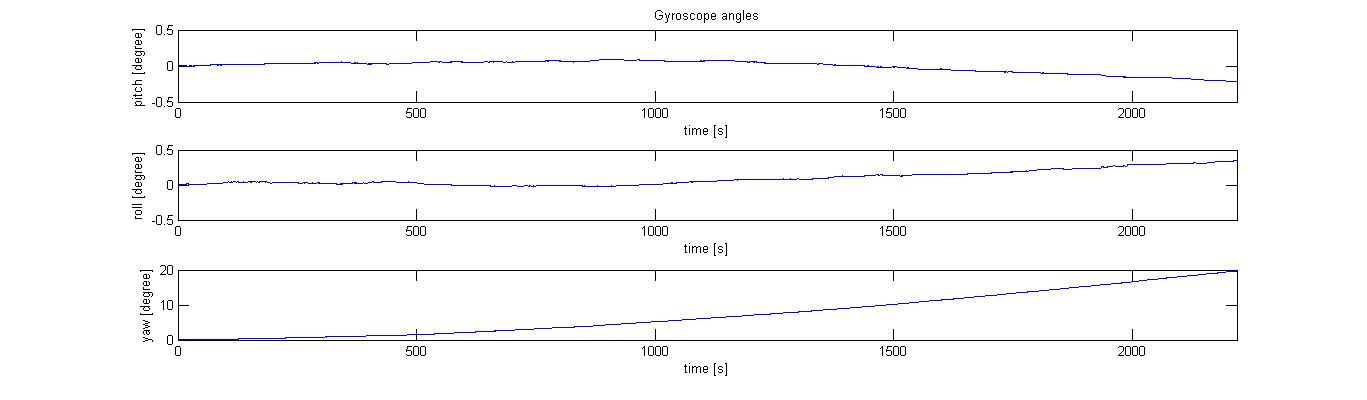
\includegraphics[width=1.0\textwidth]{fig/Comp_gyro.jpg}
	\caption{Gyroscope angles}
	\label{fig:Comp_gyro}
\end{figure}

To use all positive features of the sensors and reduce the negative drawbacks a sensor fusion is the needed solution. There are many possibilities for fusion algorithms. In this project a Complementary-Filter and Kalman-Filter is implemented.

